% !TeX root = ../thuthesis-example.tex

\chapter{实验章节}

本章将对前文所提出的高可用和容错能力进行实验,验证这些设计的效果。本章首先介绍实验环境,然后验证故障检测和判断能力,包括Phi Accrual研判算法的特性、和固定超时研判的比较、非对称网络分区和进程宕机场景下的检测能力。
然后再验证共识模块的三种协议在可用性上的表现,包括\failover 的速度、故障期间的性能和恢复的速度。
最后,本章节将会验证在进程宕机、磁盘写满、网络分区、集群变更等常见故障场景下的RTO和RPO数据。


\section{实验环境}


\begin{table}[h!]
    \centering
    \caption{服务器 环境}
    \label{tab:server_environment}
    \begin{tabular}{ll}
        \toprule
        配置 名称 & 配置 描述 \\
        \midrule
        CPU & Intel ( R ) Core ( TM ) i7-10700 CPU @ 2.90GHz 8 核 16 线程 \\
        内存 & 32GB \\
        磁盘 & 10TB HDD ( Seagate ST10000NM001G - 2MW103 ) \\
        网络 & 千兆 网卡 ( 1000Mb / s ) \\
        操作系统 & Ubuntu 20.04.5 LTS \\
        Java 版本 & OpenJDK 11.0.32 \\
       数据节点运行内存 & 28GB \\
       管理节点运行内存 & 2GB \\
        \bottomrule
    \end{tabular}
\end{table}

表格\ref{tab:server_environment}展示了测试所用的硬件环境和软件环境。测试机器分为4台,配置均为表格中展示的一致,三台用于运行IoTDB数据节点,一台用于运行IoTDB管理节点和测试程序。数据节点
分配了 28 GB 的内存,管理节点 分配了 2 GB 的内存。IoTDB 使用了一块希捷
ST-16000NM000J 机械硬盘作为存储设备,系统数据、写前日志、系统运行日志等
都会存储在同一块磁盘上。 IoTDB 使用了 OpenJDK 11.0.22 作为运行环境,操作系
统为 Ubuntu 20.04.2 LTS,64 位。测试机器之间的网络通过 1000 Mbps 的局域网连
接。

本文使用IoT-Benchmark\cite{iot-benchmark}模拟用户的写入负载。如无特殊说明,本章节所有实验所使用的IoT-Benchmark的配置如表格\ref{tab:iot-benchmark-default}所示。

\begin{table}[h!]
    \centering
    \caption{本章节测试所用IoT Benchmark配置}
    \label{tab:iot-benchmark-default}
    \begin{tabular}{ll}
        \toprule
        配置 名称 & 配置值 \\
        \midrule
        设备 数 & 100000  \\
        每个设备的序列数 & 10   \\
        存储组数 & 5  \\
        写入客户端数 & 25  \\
        每个写入请求的设备数 & 1000  \\
        每个写入请求中每个设备的记录数 & 1 \\
        \bottomrule
    \end{tabular}
\end{table}

\section{故障场景的RTO和RPO情况}

本节测试了\ref{chap-failure-scenarios}章节中描述的常见错误场景的RTO和RPO情况。
本节测试部署了3个管理节点和3个数据节点,分别使用3个IoT-Benchmark向3个数据节点写入数据,通过模拟故障的发生,来获取集群在故障时期的RPO/RTO表现和整体的性能数据。本节测试中,
管理节点和数据节点之间的心跳交换间隔为1秒,数据节点之间对等心跳的交换间隔为5秒,为了减少随机超时对测试结果的影响,本节将RatisConsensus的选举最小超时设置为2.9秒,最大超时设置为3.1秒。Phi Accrual检测器的阈值为30,可容忍的最大暂停为10秒。


本节设计的吞吐计算方法为三个Benchmark给出的端到端吞吐的平均值。
本节设计的RPO计算方法为:当故障发生且Benchmark写入结束之后,使用客户端查询集群中的数据数量,并与Benchmark写入的数据数量进行比较。
本节设计的RTO计算方法为:当故障发生之后,连接在故障节点的Benchmark从请求发出到该请求最终成功执行所需要的时间。


\begin{table}[h!]
    \centering
    \caption{不同故障下的RPO表现}
    \label{tab:exp-rpo-overview}
    \begin{tabular}{@{}lllll@{}}
        \toprule
        故障 & RatisConsensus & IoTConsensus & IoTConsensusV2 \\
        \midrule
        磁盘写满 & 0 & 0 & 0  \\
        进程宕机 & 0 & 0 & 0  \\
        对称网络分区 & 0 & 0 & 0  \\
        非对称网络分区 & 0 & 0 & 0  \\
        集群变更 & 0 & 0 & 0  \\
        \bottomrule
    \end{tabular}
  \end{table}

表\ref{tab:exp-rpo-overview}给出了集群的RPO表现。实验证明在上述的故障中,IoTDB成功做到了RPO为零的目标。这意味着数据一旦在IoTDB集群提交,IoTDB能够保证数据不会丢失。



  \begin{table}[h!]
    \centering
    \caption{不同故障下的RTO表现}
    \label{tab:exp-rto-overview}
    \begin{tabular}{@{}lllll@{}}
        \toprule
        故障 & RatisConsensus & IoTConsensus & IoTConsensusV2 \\
        \midrule
        磁盘写满 & 3.30s & 0.99s & 1.04s \\
        进程宕机 & 3.05s & 0.21s & 0.19s \\
        对称网络分区 & 13.72s & 14.10s & 13.88s \\
        非对称网络分区 & 59.90s & 60.04s & 61.99s \\
        集群变更 & 0 & 0 & 0 \\
        \bottomrule
    \end{tabular}
  \end{table}

表\ref{tab:exp-rto-overview}给出了集群的RTO表现。实验证明在上述的故障中,IoTDB的RTO在秒级到分钟级的范围内。


\subsection{磁盘写满}

磁盘写满故障的测试方法为:保持IoTDB集群运行,在第30s内手动设置一个数据节点为只读,观察benchmark写入的吞吐变化。


\begin{figure}
    \centering
    \includegraphics[width=0.99\linewidth]{exp-rto-rpo-diskfull.png}
    \caption{磁盘写满故障下的集群吞吐表现}
    \label{fig:exp-rto-rpo-diskfull}
\end{figure}

图\ref{fig:exp-rto-rpo-diskfull}给出了磁盘写满故障下的集群吞吐表现。
实验结果表明,对于IoTConsensus和IoTConsensusV2来说,故障会导致约1/3的吞吐下降,但在1s时间之后集群会通过自动容错恢复吞吐,恢复后的吞吐约为最初的80\%。
对于RatisConsensus来说,如果磁盘写满的是领导者副本,故障会导致约3s的不可用,随后集群吞吐逐渐恢复。如果磁盘写满的是Follower副本,那么故障只会导致吞吐约1/3的下降,同样在1s之后通过自动容错恢复吞吐。恢复后的吞吐约为最初的90\%。

\subsection{进程宕机}

进程宕机故障的测试方法为:保持IoTDB集群运行,在第30s的时候通过操作系统的kill -9命令强制关闭一个数据节点进程,观察benchmark写入的吞吐变化。


\begin{figure}
    \centering
    \includegraphics[width=0.99\linewidth]{exp-rto-rpo-process-down.png}
    \caption{进程宕机故障下的集群吞吐表现}
    \label{fig:exp-rto-rpo-process-down}
\end{figure}

图\ref{fig:exp-rto-rpo-process-down}给出了磁盘写满故障下的集群吞吐表现。
实验结果表明,对于IoTConsensus和IoTConsensusV2来说,故障会导致约1/3的吞吐下降,但在200毫秒时间之后集群会通过自动容错恢复吞吐。对于RatisConsensus来说,如果磁盘写满的是领导者副本,故障会导致约3s的不可用,随后集群吞吐逐渐恢复。如果磁盘写满的是Follower副本,那么故障只会导致吞吐约1/3的下降,同样在200毫秒之后通过自动容错恢复吞吐。


\subsection{对称网络分区}
对称网络分区故障的测试方法为:保持IoTDB集群运行,在第60s的时候配置iptable使其中一个节点和剩下两个节点之间的网络都不可达,观察benchmark写入的吞吐变化。


\begin{figure}
    \centering
    \includegraphics[width=0.99\linewidth]{exp-rto-rpo-sym-network-partition.png}
    \caption{对称网络分区故障下的集群吞吐表现}
    \label{fig:exp-rto-rpo-sym-network-partition}
\end{figure}

图\ref{fig:exp-rto-rpo-sym-network-partition}给出了对称网络分区故障下的集群吞吐表现。
结果表明,在实验运行的时间里,对称网络分区对IoTConsensus和IoTConsensusV2两个共识协议的吞吐未产生明显的影响。对于RatisConsensus而言,故障会导致吞吐约1/3的下降,直到15秒之后才会逐渐恢复。

\subsection{非对称网络分区}

非对称网络分区故障的测试方法为:保持IoTDB集群运行,在第60s的时候配置iptable使其中两个节点之间的网络不可达,观察benchmark写入的吞吐变化。


\begin{figure}
    \centering
    \includegraphics[width=0.99\linewidth]{exp-rto-rpo-asym-network-partition.png}
    \caption{非对称网络分区故障下的集群吞吐表现}
    \label{fig:exp-rto-rpo-asym-network-partition}
\end{figure}

图\ref{fig:exp-rto-rpo-asym-network-partition}给出了非对称网络分区故障下的集群吞吐表现。
结果表明,在实验运行的时间里(10分钟),非对称网络分区对IoTConsensus和IoTConsensusV2两个共识协议的吞吐未产生明显的影响。对于RatisConsensus而言,故障会导致吞吐约1/3的下降,直到60秒之后才会逐渐恢复。

\subsection{集群变更}

集群变更场景下的RPO/RTO的测试方法为:保持IoTDB集群运行,持续运行扩容脚本和缩容脚本,将数据节点的数量不断从3个扩容成4个,再从4个缩容成3个,持续这个过程,观察benchmark写入的吞吐变化。


\begin{figure}
    \centering
    \includegraphics[width=0.99\linewidth]{exp-rpo-rto-conf-change.png}
    \caption{集群变更阶段的吞吐表现}
    \label{fig:exp-rpo-rto-conf-change}
\end{figure}

图\ref{fig:exp-rpo-rto-conf-change}给出了集群变更阶段的吞吐表现。
实验结果表明,集群变更并没有对集群和RTO有明显的影响。对于RatisConsensus来说,集群变更导致了整体吞吐约5\%的略微下降。

\subsection{管理节点脑裂}

管理节点脑裂场景的测试方法为:保持IoTDB集群运行,通过iptable命令,让管理节点领导者和其他两个管理节点之间出现对称网络分区,持续观察共识协议的选举日志,保证下一轮领导者的选举成功时间晚于被分区的领导者的下线时间。

在实验中,我们将领导者的租约有效时间设置为最短超时时间的80\%。在100次实验中,观察到下一轮领导者的选举成功时间早于被分区的领导者的下线时间的实验次数为0次。下一轮领导者的选举成功实践平均晚于上一轮领导者的下线时间590ms。

实验结果表明,通过将领导者的租约时间设置为低于最短超时时间,并将管理节点的客户端超时时间设置为大于选举超时,我们能够保证管理节点的服务不出现脑裂的问题,同时通过重试的方式避免因管理节点服务短暂不可用导致的请求失败。

\subsection{和TDengine的对比}

对于\ref{chap-failure-scenarios}章节中描述的常见错误场景的RTO和RPO情况,
表\ref{tab:exp-rto-compare-tdengine}给出了TDengine系统的RTO表现。

对比测试的实验方法为:部署一个3个mnode、3个dnode的TDengine集群,其他参数采用默认,其中Raft的选举时长为20-25s。使用3个IoT-Benchmark按照\ref{tab:iot-benchmark-default}的负载分别连接3个dnode写入数据。IoTDB的对照组采用RatisConsensus协议,RTO的计算方法采取上述的黑箱方式。

\begin{table}[h!]
    \centering
    \caption{和TDengine的RTO对比}
    \label{tab:exp-rto-compare-tdengine}
    \begin{tabular}{@{}lllll@{}}
        \toprule
        故障 & RatisConsensus & TDEngine \\
        \midrule
        磁盘写满(无负载/有负载) & 6.30s/0.08s & NA/0.10s \\
        进程宕机 & 6.05s & 21.09s \\
        对称网络分区 & 13.72s & 36.88s \\
        非对称网络分区 & 59.90s & 39.20s \\
        集群变更 & 0 & 0 \\
        \bottomrule
    \end{tabular}
  \end{table}

在磁盘写满的故障中,如果有实时的写入负载,IoTDB和TDengine都能够在磁盘写满后的下一次写入操作检测出故障并上报。然而,在无负载的情况下,IoTDB可以主动识别磁盘写满的故障并触发领导者选举,在平均6.30s实现故障的切换和恢复,TDengine则没有这样的机制。

在主副本进程宕机的故障中,IoTDB的RTO表现要优于TDengine。这是由两者的默认Raft选举超时参数决定的。由于主副本宕机后,集群需要经过一个选举超时才能出现新的领导者副本,因此,不可用的时间和选举超时成正比。

TDengine在对称分区和非对称分区两种网络分区场景下表现较为稳定,由于其重客户端的原因,所以两个故障的RTO都是在半分钟左右。

IoTDB的对称网络分区故障的恢复速度相较更快,但非对称分区故障恢复速度相对较慢。由于非对称分区故障的实际出现概率不高,所以IoTDB在相关参数上降低了非对称分区故障的检测频率,用相对更长的恢复速度换取了更低的后台检测开销。


\section{故障检测}

\subsection{非对称网络分区故障的检测}

在本小节中,我们测试了IoTDB对于非对称网络分区的检测能力。

测试方法如下:设置IoTDB的Phi Accrual故障阈值为30,数据节点之间的对等心跳频率为5s一次,在节点平稳运行后的120s之后,使用防火墙iptables的命令阻断其中两个数据节点之间的通信,模拟非对称网络分区的故障,计时记录管理节点领导者研判集群出现非对称网络分区的速度。使用自动化工具重复上述过程1000次。

\begin{figure}
    \centering
    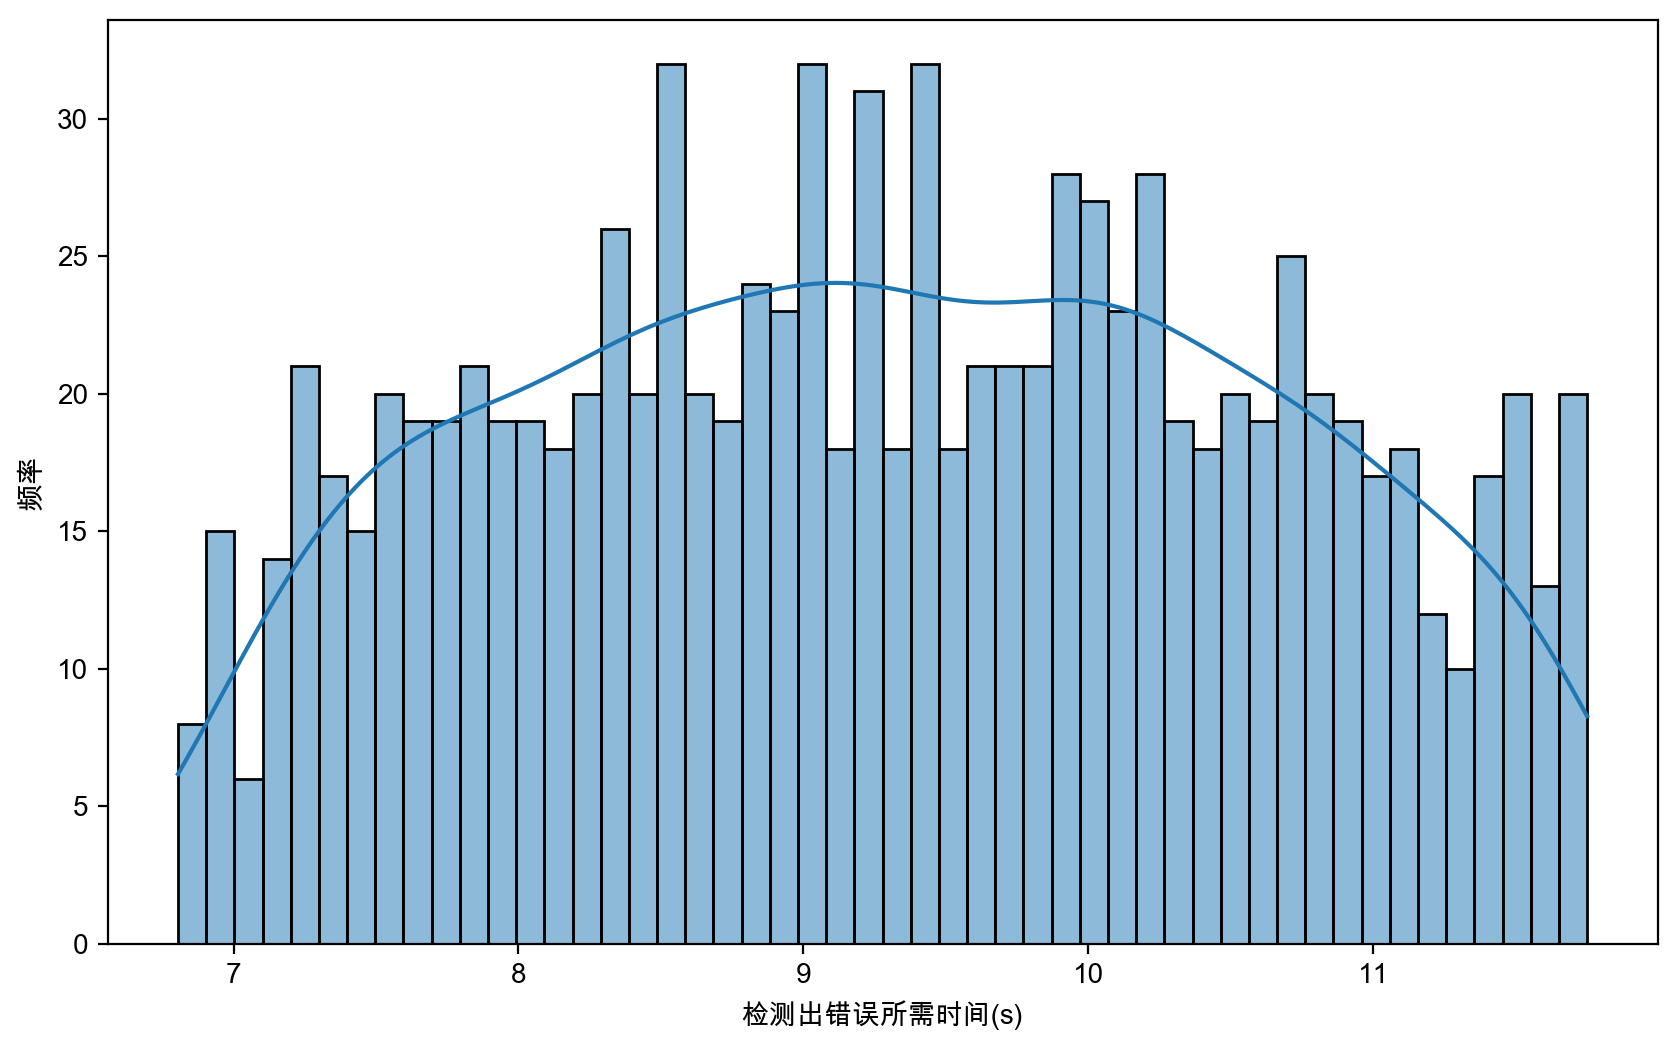
\includegraphics[width=0.8\linewidth]{exp-asym-np-detect.png}
    \caption{非对称网络分区检测故障所需时间的分布}
    \label{fig:exp-asym-np-detect}
\end{figure}

图\ref{fig:exp-asym-np-detect}展示了1000次实验中非对称网络分区检测所需时间的分布。1000次实验中,管理节点领导者无一例外全部检测到了非对称网络分区,平均的检测用时是9.30s,检测用时的标准差是2.08s。

\begin{figure}
    \centering
    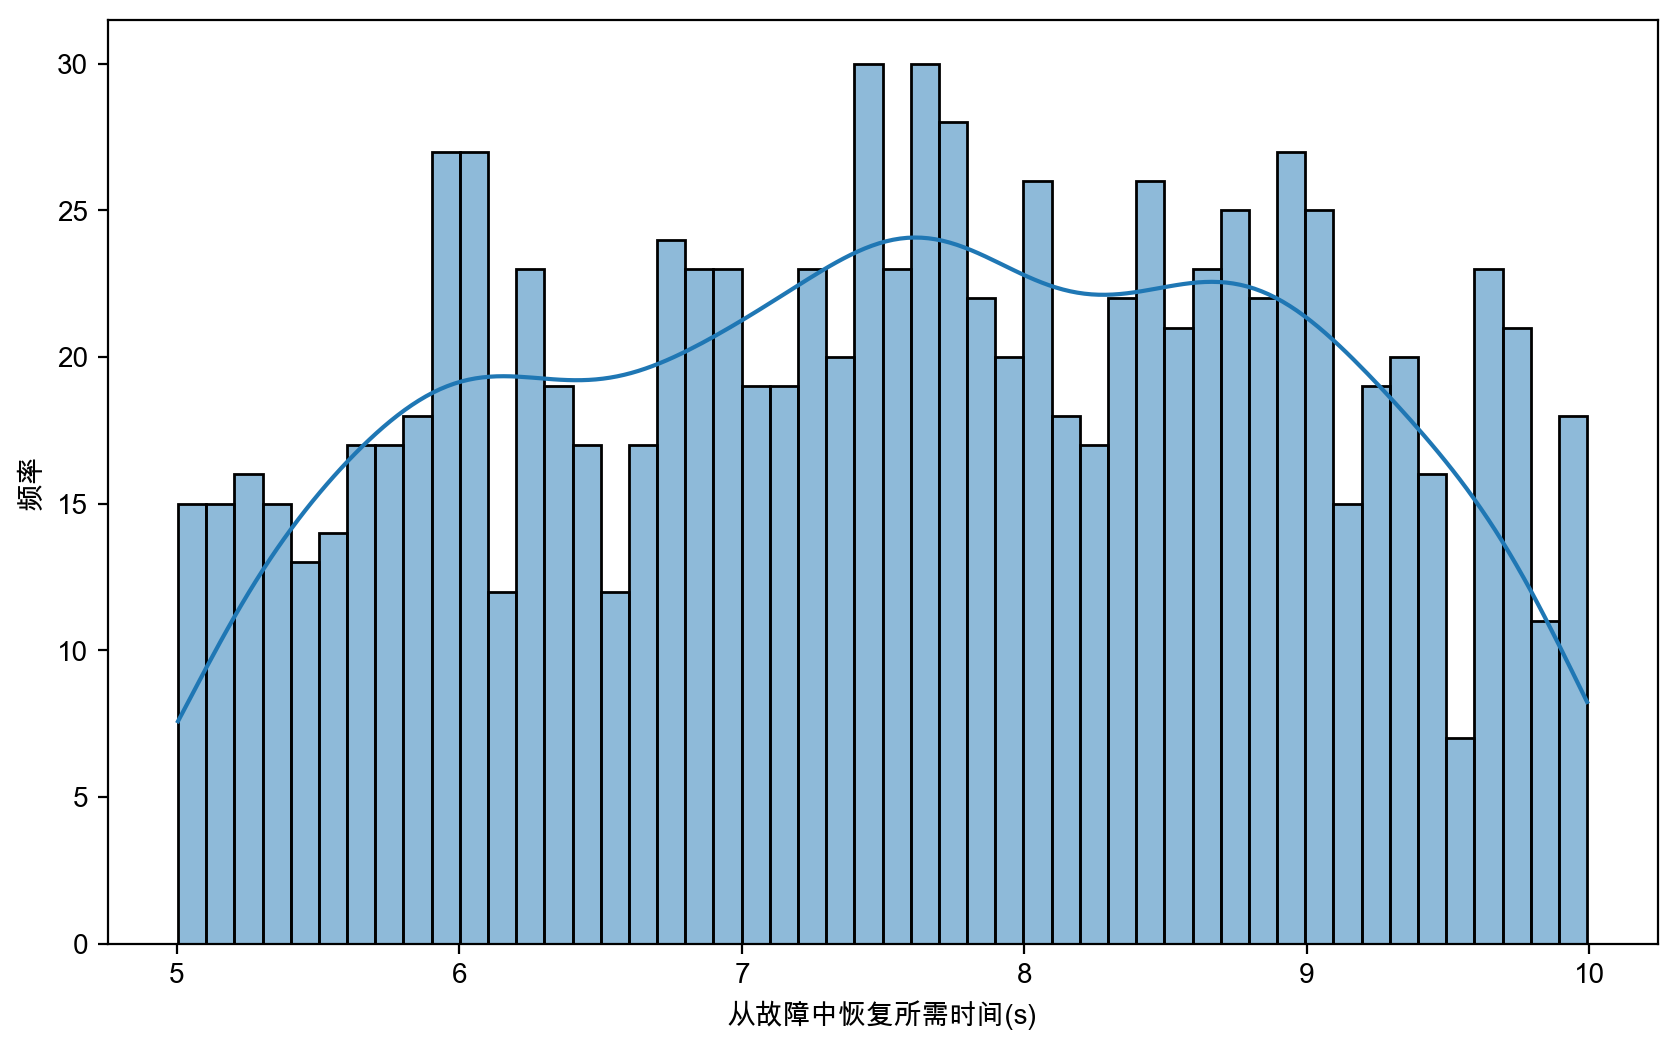
\includegraphics[width=0.8\linewidth]{exp-asym-np-recover.png}
    \caption{非对称网络分区检测恢复所需时间的分布}
    \label{fig:exp-asym-np-recover}
\end{figure}

在检测到非对称网络分区的120s后,解除防火墙的阻断,计时记录管理节点领导者研判集群不再具有非对称网络分区故障的时间。图\ref{fig:exp-asym-np-recover}展示了1000次实验中检测出非对称网络分区问题已恢复所需时间的分布。1000次实验中,管理节点领导者无一例外全部检测到了系统从非对称网络分区的故障中恢复,平均的检测用时为7.55s,检测用时的标准差是2.45s。

实验结果表明,IoTDB集群通过数据节点之间的对等心跳机制能够有效对非对称网络分区问题进行检测,且检测所需的时间在几秒到几十秒的范围内。当非对称网络分区结束后,心跳一经联通,IoTDB也会立即研判非对称网络分区问题结束。


\subsection{Phi Accrual故障研判算法的行为表现}\label{sec-experience-phi-accrual}

\subsubsection{算法的参数行为}

本文前面章节提出的基于Phi Accrual算法的故障检测机制具有两个可指定参数。
参数一是预设的故障检测阈值,默认为30。Phi Accrual算法会通过心跳的到达间隔采样窗口,计算节点的可能故障概率的指数量化指标Phi,并跟预设的故障检测阈值进行比较,给出故障研判的结果。
参数二是可容忍的最大心跳暂停,默认为10s。在JVM环境中,由于垃圾回收的机制可能导致进程暂停,因此对应的心跳也会暂停。为了容忍这种暂停,避免其影响研判的正确率,Phi Accrual允许设置最大的暂停时间。

本节给出了Phi Accrual在不同的参数下的行为表现。

\begin{figure}
    \centering
    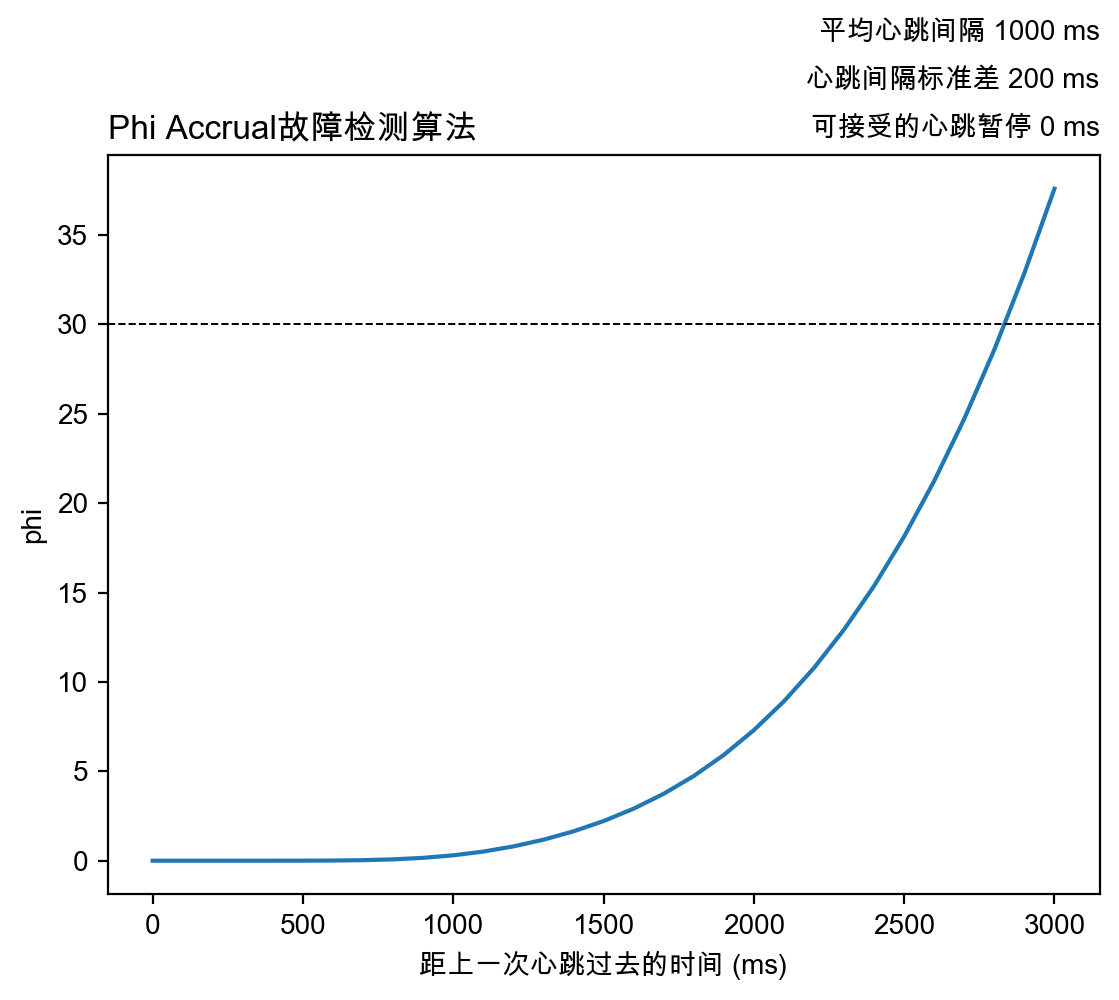
\includegraphics[width=0.6\linewidth]{exp-phi.png}
    \caption{Phi值随上一次心跳时间间隔变化示意图}
    \label{fig:exp-phi}
\end{figure}

图\ref{fig:exp-phi}展示了算法的故障概率量化指标Phi随着最后一次心跳经过的时间的变化情况。
在本次测试中,平均心跳之间的到达间隔约为1000ms,到达间隔的标准差固定为200ms,可容忍的最大心跳暂停为0。

实验结果表明了Phi Accrual算法能够在心跳长期未到达之后迅速给出故障预警。在距离最后一次心跳经过的时间范围不超过1000ms的时候,Phi值极低,接近零,代表此时算法研判的故障概率很低。超过1000ms之后,Phi值会随着最后一次心跳经过的时间呈指数型迅速升高,并在约2700ms的时候达到IoTDB的预设阈值30。这意味着如果2700ms没有接收到该有的心跳,Phi Accrual故障检测算法就会研判该节点出现了故障,这种检测效率远远高于原先的20s固定心跳超时。


\begin{figure}
    \centering
    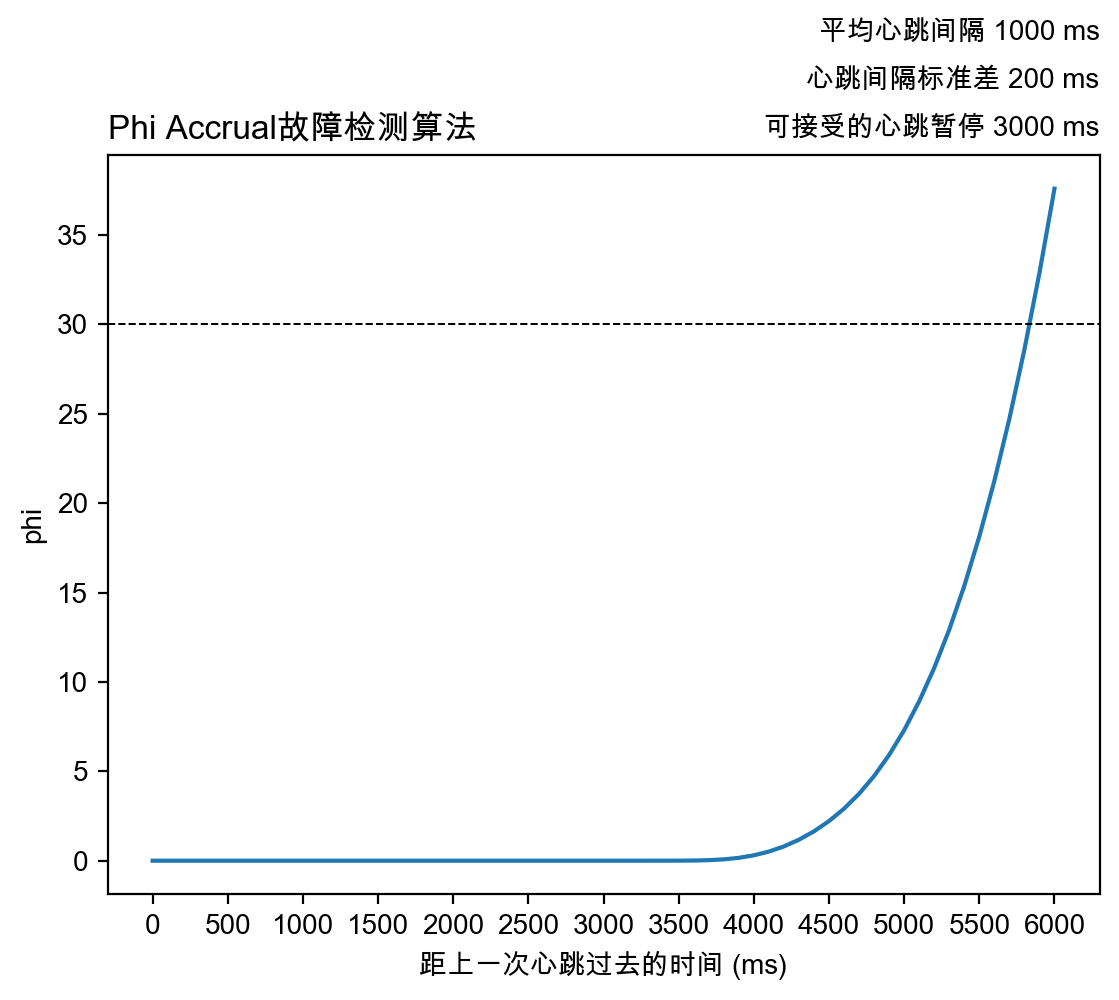
\includegraphics[width=0.6\linewidth]{exp-phi-with-pause.png}
    \caption{Phi值随上一次心跳时间间隔变化(带心跳暂停)示意图}
    \label{fig:exp-phi-with-pause}
\end{figure}

图\ref{fig:exp-phi}展示了可容忍的最大心跳暂停时间对于故障研判的影响。
在本次测试中,平均心跳之间的到达间隔约为1000ms,到达间隔的标准差固定为200ms,可容忍的最大心跳暂停为3000ms。

实验结果表明了,Phi Accrual算法能够较好地容忍JVM垃圾回收造成的进程暂停等情况。可容忍的最大心跳暂停时间这一参数能够线性地影响Phi值的计算。在距离最后一次心跳经过的时间范围不超过4000ms的时候,Phi值极低,接近零,代表此时算法研判的故障概率很低。超过4000ms之后,Phi值会随着最后一次心跳经过的时间呈指数型迅速升高,并在约6700ms的时候达到IoTDB的预设阈值30。相较于上一组实验,每一个关键节点都朝右偏移了3000ms,表明了Phi值计算受可容忍的最大心跳暂停时间线性影响的特点。


\subsection{Phi Accrual和固定超时算法检测能力对比}
本小节比较了基于Phi Accrual的故障检测算法和基于固定超时的故障检测算法在现实场景中的故障检测能力。场景包括正常运行场景、高负载场景、负载呈周期性变化场景、负载逐渐升高场景,故障检测能力的指标是平均故障发现时间和平均的误报次数。

本节的测试通过使用用户负载模拟程序IoT Benchmark实现,不同场景的Benchmark的配置参数如表\ref{tab:extended_columns}所示,表格中的t代表运行的时间,单位是分钟。

\begin{table}[h!]
    \centering
    \caption{不同负载场景的IoT Benchmark配置}
    \label{tab:extended_columns}
    \begin{tabular}{lllll}
        \toprule
        配置 名称 & 正常负载 & 高负载 & 周期负载 & 负载逐渐升高 \\
        \midrule
        设备 数 & 100000 & 100000 & 100000 & 100000 \\
        每个设备的序列数 & 10 & 10 & 10 & 10  \\
        存储组数 & 5 & 5 & 5 & 5 \\
        写入客户端数 & 25 & 25 & 25 & 25 \\
        每个写入请求的设备数 & 1000 & 1000 & 1000 & 1000 \\
        每个写入请求中每个设备的记录数 & 1 & 10 & 1 + 20*(t mod 2) & 1 + max(t/20,20) \\
        \bottomrule
    \end{tabular}
\end{table}

本节测试的参数选择:管理节点和数据节点之间交换心跳的间隔为1s,固定心跳超时被设置在20s,Phi Accrual的超时阈值在30,可容忍的最大心跳暂停为10s。

\begin{table}[h!]
    \centering
    \caption{正常运行场景下的固定超时和Phi Accrual算法对比}
    \label{tab:exp-normal-load}
    \begin{tabular}{@{}llll@{}}
        \toprule
        场景 & 算法 & 平均故障发现延迟 (s) & 平均误报次数(100次中) \\
        \midrule
        正常运行 & 固定心跳超时 & \SI{20.02}{\second} & 0 \\
        正常运行 & Phi Accrual & \SI{13.85}{\second} & 0 \\
        \bottomrule
    \end{tabular}
\end{table}

表\ref{tab:exp-normal-load}给出了正常运行场景下固定超时算法和Phi Accrual算法的对比。
实验方法如下:运行在持续运行120s之后,按照50\%的概率杀死一个进程,接着记录两个算法发现故障的平均延迟和误报情况。在本场景下GC暂停的时间通常不超过1s。
实验结果表明了,在正常运行期间,Phi Accrual相较于固定心跳超时能够更快地检测出错误,两者在不受GC暂停的影响下误报率都非常的低。


\begin{table}[h!]
    \centering
    \caption{高负载运行场景下的固定超时和Phi Accrual算法对比}
    \label{tab:exp-high-load}
    \begin{tabular}{@{}llll@{}}
        \toprule
        场景 & 算法 & 平均故障发现延迟 (s) & 平均误报次数(100次中) \\
        \midrule
        高负载运行 & 固定心跳超时 & \SI{20.09}{\second} & 5 \\
        高负载运行 & Phi Accrual & \SI{22.80}{\second} & 1 \\
        \bottomrule
    \end{tabular}
\end{table}

表\ref{tab:exp-high-load}给出了高负载运行场景下固定超时算法和Phi Accrual算法的对比。
实验方法如下:运行在持续运行120s之后,按照50\%的概率杀死一个进程,接着记录两个算法发现故障的平均延迟和误报情况。在本场景下GC暂停的总时间达到总CPU时间的20\%,单次GC暂停的时间从一秒到十几秒不等。
实验结果表明了,在高负载运行场景下,
Phi Accrual的检测速度略微低于固定心跳,但是误报率大大下降,达到了发现延迟和误报率的较好的一个平衡。如果GC暂停的时间远大于固定超时20s,那么固定心跳超时的误报率将会呈直线上升的趋势。


\begin{table}[h!]
    \centering
    \caption{负载逐渐提高场景下的固定超时和Phi Accrual算法对比}
    \label{tab:exp-increase-load}
    \begin{tabular}{@{}llll@{}}
        \toprule
        场景 & 算法 & 平均故障发现延迟 (s) & 平均误报次数(100次中) \\
        \midrule
        负载逐渐提高 & 固定心跳超时 & \SI{20.08}{\second} & 17 \\
        负载逐渐提高 & Phi Accrual & \SI{24.45}{\second} & 4 \\
        \bottomrule
    \end{tabular}
\end{table}

表\ref{tab:exp-increase-load}给出了负载逐渐提高运行场景下固定超时算法和Phi Accrual算法的对比。
实验方法如下:运行在持续运行120s之后,按照50\%的概率杀死一个进程,接着记录两个算法发现故障的平均延迟和误报情况。在本场景下GC暂停的总时间达到总CPU时间的27\%,单次GC暂停的时间从一秒到几十秒不等。随着测试时间的增加,GC暂停的频率和时长都有所增加。

实验结果表明了,在负载逐渐提高运行场景下,
Phi Accrual和固定心跳超时的误报率都有所上升,但Phi Accrual的误报率依然远低于固定心跳超时。两者的检测速度依然相似,Phi Accrual的故障发现延迟略微低于固定心跳。


\begin{table}[h!]
    \centering
    \caption{负载周期行变化场景下的固定超时和Phi Accrual算法对比}
    \label{tab:exp-seasonal-load}
    \begin{tabular}{@{}llll@{}}
        \toprule
        场景 & 算法 & 平均故障发现延迟 (s) & 平均误报次数(100次中) \\
        \midrule
        负载周期变化 & 固定心跳超时 & \SI{19.98}{\second} & 11 \\
        负载周期变化 & Phi Accrual & \SI{23.20}{\second} & 2 \\
        \bottomrule
    \end{tabular}
\end{table}

表\ref{tab:exp-high-load}给出了负载周期变化运行场景下固定超时算法和Phi Accrual算法的对比。
实验方法如下:运行在持续运行120s之后,按照50\%的概率杀死一个进程,接着记录两个算法发现故障的平均延迟和误报情况。在本场景下GC暂停的总时间达到总CPU时间的25\%,单次GC暂停的时间从一秒到几十秒不等,GC暂停的时间和频率能够观察到周期性变化,但略微落后于负载的周期性变化。

实验结果表明了,在负载周期变化场景下,
Phi Accrual依然保持了非常良好的动态调整能力,误报率依然保持在很低的水平。Phi Accrual的检测速度略微低于固定心跳,但实际差距并不明显。

总结来说,通过模拟四种不同负载的场景,我们能够得出以下结论:Phi Accrual算法在正常场景下有着更快的故障检测速度,并且展现出了出了随着系统实际负载变化而变化的自适应能力,在负载较高或者负载变化的场景下能够以牺牲微量检测时延的代价获得极低的误报率。


\subsection{基于Thrift连接的进程宕机检测速度}

\begin{table}[h!]
    \centering
    \caption{进程宕机情况下故障发现优化实验}
    \label{tab:exp-thrift-process-down}
    \begin{tabular}{@{}llll@{}}
        \toprule
        场景 & 算法 & 平均故障发现延迟 (s) \\
        \midrule
        进程宕机 & 基于心跳和研判算法 & \SI{13.72}{\second}  \\
        进程宕机 & 基于Thrift连接状态 & \SI{0.05}{\second}  \\
        \bottomrule
    \end{tabular}
\end{table}

表\ref{tab:exp-thrift-process-down}给出了基于Thrift连接的进程宕机故障发现的优化验证。保持故障检测算法Phi Accrual的默认参数检测阈值为30,管理节点和数据节点的心跳间隔为1s。

实验结果表明,基于Thrift连接状态的主动通知型故障检测的延迟显著低于基于心跳历史的研判算法。


\section{副本和共识协议}

\subsection{故障后的容错表现}

本小节测试了三种共识协议在副本发生故障之后的容错表现。测试方法如下:为每一个协议配置三个副本,使用三个IoT-Benchmark分别向三个副本写入,并在运行一段时间之后手动关闭一个副本,模拟副本故障的情况,并且保持写入,衡量前后的吞吐变化。客户端在发现故障后重试的配置参数为3次,每次需要等待1s才会执行。RatisConsensus的副本选举时间设定为4s到8s之间。

\begin{figure}
    \centering
    \includegraphics[width=0.99\linewidth]{exp-consensus-failure.png}
    \caption{不同共识协议的故障容错表现}
    \label{fig:exp-consensus-failure}
\end{figure}


图\ref{fig:exp-consensus-failure}展示了测试的结果。

在故障发生之后吞吐的下降峰值是衡量共识协议可用性的一个指标。如图所示,IoTConsensus在单一副本故障之后吞吐下降了33\%,IoTConsensusV2在单一副本故障之后吞吐下降了37\%,RatisConsensus在单一副本故障之后吞吐下降了96\%。
实验结果表明,IoTConsensus和IoTConsensusV2在单一副本故障发生时有着更好的可用性,因为其他不受影响的副本可以独立服务写入请求,使得总吞吐量大约下降1/3。但是RatisConsensus在单一副本(主副本)发生故障时有一段时间的不可用,原因是共识协议需要重新选举新的主副本,在新的主副本选举完成之前所有副本都无法接受写入请求。

在故障发生之后吞吐的恢复速度是衡量共识协议错误转移速度的一个指标。
当客户端检测到节点故障之后,会通过数据节点发现和重定向的方式,将原来连接到故障节点的请求重定向到正常的节点上,从而完成写入的恢复。
如图所示,IoTConsensus和IoTConsensusV2在故障后约3-5s写入吞吐就能大致恢复,而RatisConsensus在故障后约8s写入吞吐才大致恢复。
由于重试和超时时间的设置,客户端需要至少3s才会进行请求的重定向,这跟我们的实验结果比较吻合。RatisConsensus这边多出来的时间是领导者重新选举的选举超时。

实验结果表明,IoTConsensus和IoTConsensusV2有着更极致的可用能力,在单一副本发生故障的时候的吞吐下降峰值、吞吐恢复速度两个指标上都更优于RatisConsensus。


\subsection{故障副本的恢复时间}

本小节测试了在三种不同共识协议的故障副本恢复表现。测试方法如下:为每一个协议配置三副本,使用IoT-Benchmark持续写入数据。在写入数据5分钟之后,手动结束一个副本的进程,模拟故障的发生,但保持数据继续写入其他副本。再过五分钟之后,重启这个故障的副本,测试这个故障恢复的副本从进程重启到已经同步完宕机期间所有数据所需要的时间。IoTConsensusV2使用数据同步百分比代表追赶进度,IoTConsensus使用WAL的index代表追赶进度,而RatisConsensus使用Raft Term和Index代表追赶进度。

\begin{figure}[!t]
    \centering
    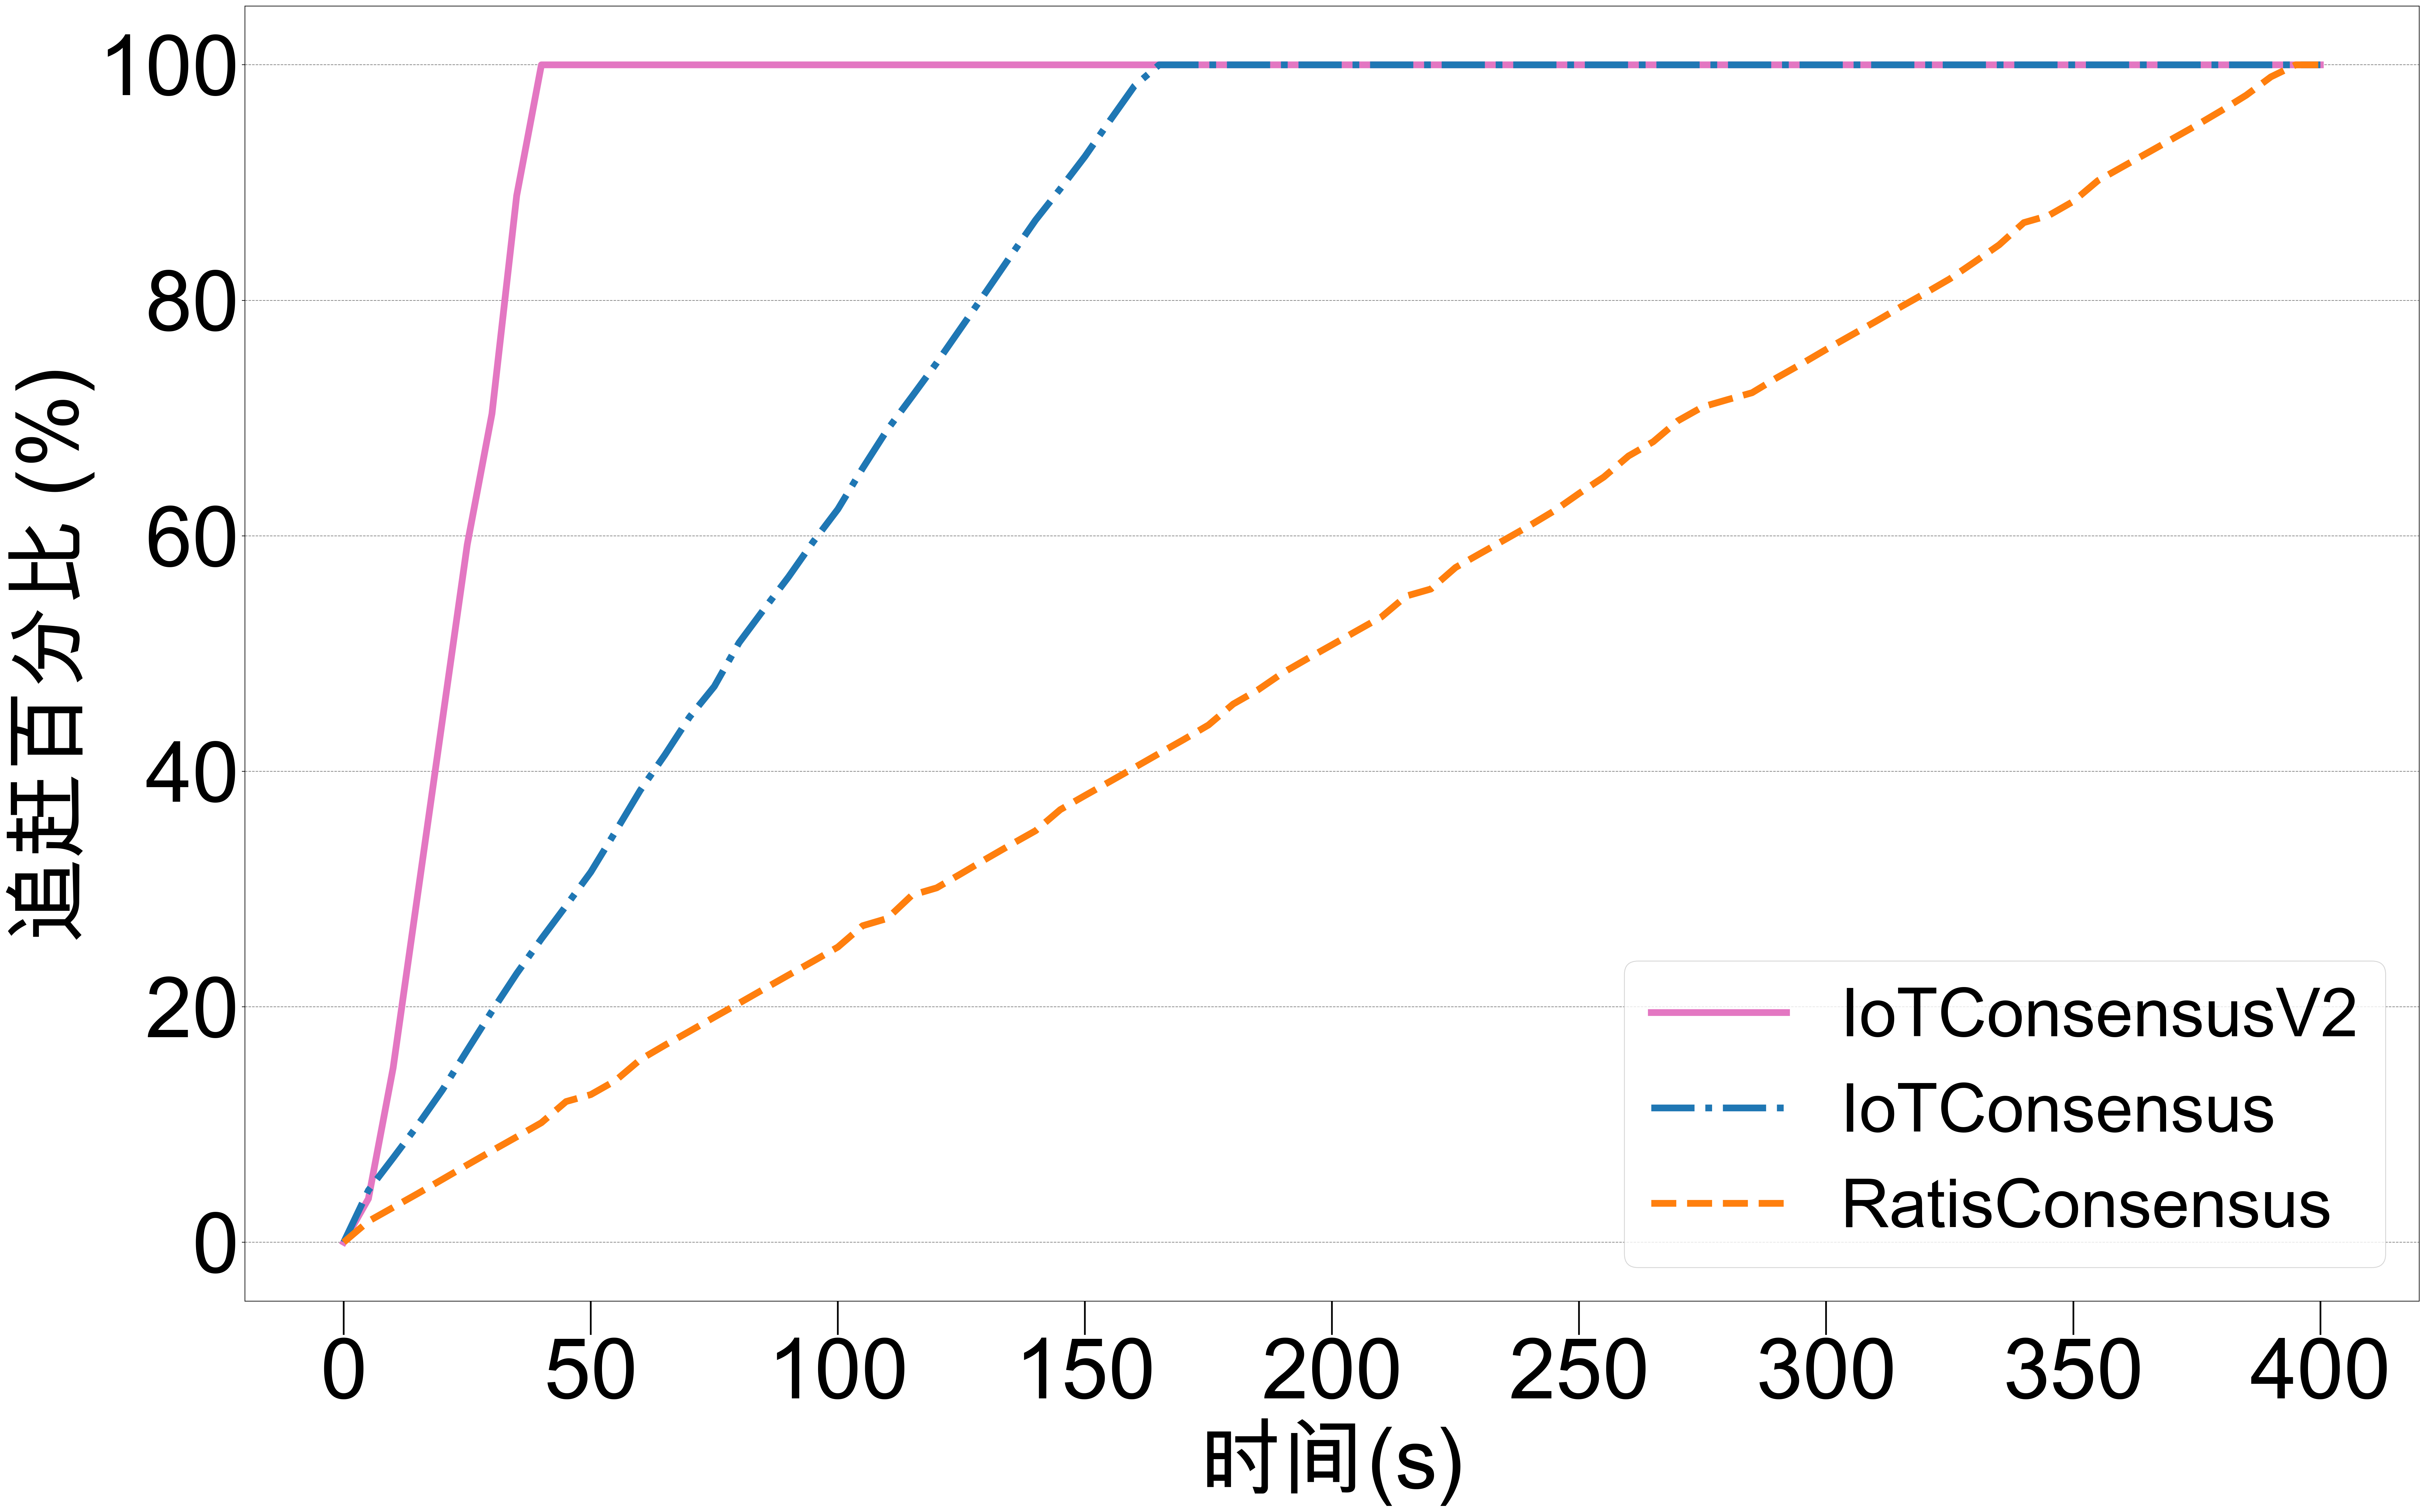
\includegraphics[width=0.8\linewidth]{exp-catch-up.png}
    \caption{不同共识协议的故障副本恢复表现}
    \label{fig:exp-catch-up}
\end{figure}

图\ref{fig:exp-catch-up}展示了实验的结果。在重启之后,IoTConsensusV2使用了40s的时间同步完了宕机期间的数据,IoTConsensus使用了170s的时间完成同步,而RatisConsensus使用了390s的时间完成同步。

实验结果表明,三种共识协议都能够自动恢复故障的副本。由于IoTConsensusV2通过TsFile进行数据传输,在恢复速度上显著优于IoTConsensus和RatisConsensus。


% \section{和其他数据库的RTO和RPO对比}

% 给出端到端的一个比较吧

% IoTDB
% TimeScale DB 
% tdengine
% opentsdb
% Oceanbase